% ==========================================================
% 关键修复:在加载类之前,强行指定 ctex 使用 fandol 字体集
% 这样可以覆盖掉 ctex 在 Windows 下默认寻找 SimHei 的行为
% ==========================================================
\PassOptionsToPackage{fontset=fandol}{ctex}

% ==========================================================
% 文件路径: tex/demo/main.tex
% ==========================================================
\documentclass[lang=cn, chinesefont=ctexfont, bibend=bibtex]{elegantpaper}

% 引入你上传的自定义样式 (假设 custom.sty 和 main.tex 在同一目录,或已被安装)
% 注意:如果 custom.sty 在同级目录,直接引用即可
\usepackage{custom}

\usepackage{tikz}

% ==========================================================
% 0. 自动生成参考文献数据 (.bib)
%    这样就不需要手动上传 ref.bib 文件了,方便测试
% ==========================================================
\begin{filecontents}[overwrite]{ref.bib}
@article{tinytex,
  title   = {TinyTeX: A lightweight, cross-platform, and easy-to-maintain LaTeX distribution based on TeX Live},
  author  = {Xie, Yihui},
  journal = {TUGboat},
  volume  = {40},
  number  = {1},
  pages   = {30--32},
  year    = {2019}
}
@book{latexbook,
  title     = {LaTeX 入门},
  author    = {刘海洋},
  year      = {2013},
  publisher = {电子工业出版社},
  address   = {北京}
}
\end{filecontents}

% 添加参考文献资源
\addbibresource{ref.bib}

% ==========================================================
% 文档信息
% ==========================================================
\title{自动化环境集成测试报告}
\author{GitHub Actions}
\institute{TinyTeX CI/CD Lab}
\date{\zhtoday}

\begin{document}

\maketitle

\begin{abstract}
本文档旨在测试 \textbf{ElegantPaper} 模板在 Windows Server (GitHub Actions) 环境下的编译情况。测试覆盖了中文支持、TikZ 绘图、自定义表格样式以及参考文献生成(Biber 流程)。如果本文档编译成功且无乱码,说明 TinyTeX 环境已完全就绪。
\keywords{自动化测试; TinyTeX; ElegantPaper; 参考文献}
\end{abstract}

% ==========================================================
% 1. 字体与中文测试
% ==========================================================
\section{中文与字体测试}
当前编译环境应正确处理中文内容。我们使用 \texttt{chinesefont=ctexfont} 选项来调用 Fandol 开源字体,以适应无商业字体的服务器环境。

% ==========================================================
% 2. 自定义包功能测试 (custom.sty)
% ==========================================================
\section{自定义包测试 (custom.sty)}

\subsection{智能图片加载测试}
根据 \texttt{custom.sty} 的定义,如果图片不存在,应显示占位图并报错,而不是导致编译停止。
\begin{figure}[htbp]
    \centering
    % 这里故意引用一个不存在的图片,测试你的 Smart Graphics 系统
    \includegraphics[width=0.6\textwidth]{non-existent-image.png}
    \caption{智能图片缺省测试(应显示 Missing 红色警告)}
\end{figure}

\subsection{自定义表格样式测试}
测试 \texttt{custom.sty} 中定义的 \texttt{\textbackslash ccr} 命令:

\begin{table}[htbp]
    \centering
    \caption{自定义色块表格}
    \begin{tabular}{c c c}
        \toprule
        项目 & 颜色 & 样式示例 \\
        \midrule
        警告色 & Red & \ccr{red} \\
        强调色 & Cyan & \ccr{cyan!50} \\
        \bottomrule
    \end{tabular}
\end{table}

% ==========================================================
% 3. 绘图测试 (TikZ)
% ==========================================================
\section{绘图测试 (TikZ)}
\begin{figure}[htbp]
    \centering
    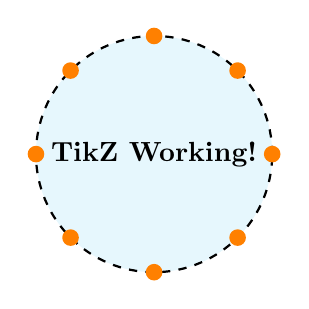
\begin{tikzpicture}
        \draw[fill=cyan!10, thick, dashed] (0,0) circle (1.5cm);
        \node at (0,0) {\textbf{TikZ Working!}};
        \foreach \angle in {0,45,...,315}
            \fill[orange] (\angle:1.5cm) circle (3pt);
    \end{tikzpicture}
    \caption{TikZ 矢量绘图测试}
\end{figure}

% ==========================================================
% 4. 引用测试
% ==========================================================
\section{引用测试}
此处测试参考文献的引用功能。如果下面的引用显示为数字(如 [1])且文末有列表,说明 Biber 工作正常。

引用一篇英文文献:TinyTeX 是一个轻量级发行版\cite{tinytex}。\\
引用一篇中文书籍:学习 LaTeX 可以参考刘海洋的书\cite{latexbook}。

% 打印参考文献
\printbibliography[heading=bibintoc, title=参考文献]

\end{document}